\chapter{Esperimenti}

    Per verificare i risultati ottenuti è stato necessario eseguire una serie di esperimenti, utili a valutare oggettivamente le prestazioni delle singole funzioni dell'algoritmo proposto.
    Tutti i test sono stati eseguiti sul mio pc personale del quale elenco le caratteristiche rilevanti:
    \begin{itemize}
        \item Processore: Intel i7 2100MhZ$\times$8
        \item Ram: 8GB
        \item GPU: NVIDIA 630m 2GB
    \end{itemize}

\section{Uso di MATLAB}
    Per la maggioranza degli esperimenti svolti sono stati utilizzati degli script in MATLAB. Grazie all'uso di questo programma è stato possibile generare velocemente immagini, permettendo in questo modo di ottenere una quantità adeguata di immagini per la procedura di testing. \'E importante notare che le immagini generate in questo modo sono esenti da rumore e contengono curve perfette.

    Un primo frammento di codice si occupa di prendere in input i parametri del percorso, grazie a delle funzioni che permettono di aggiungere uno alla volta tutti gli elementi necessari. Queste funzioni generano curve e rettilinei in base alla parte di percorso appena inserita, utilizzando come parametri lunghezza, differenza di angolazione nel caso di parti in rettilineo, o raggio e angolo di curva nel caso di elementi curvilinei.

    Una volta impostato il percorso è possibile inserire una lista di coordinate $(x, y, \alpha)$ (con $\alpha$ inteso come orientamento del robot rispetto all'asse delle $x$) e un secondo script si preoccupa di posizionare un robot immaginario sul percorso generando immagini analoghe a quelle ottenute facendo veramente muovere il robot lungo il percorso. Questo permette di velocizzare notevolmente le fasi di testing, soddisfacendo le necessità di immagini per eseguire test senza la necessità di usare effettivamente il robot.

\section{Test sulla funzione di calcolo dei parametri della curva}
    Un primo test importante da eseguire è sulla funzione che calcola i parametri della curva. Infatti, in un caso ideale,  l'algoritmo riuscirebbe a ricostruire la distanza dall'inizio della curva, il raggio e l'angolo di curvatura della stessa il più precisamente possibile.

    I test sono stati svolti su un campione di 540 immagini differenti, ognuna contenente una curva a distanze diverse comprese tra 1 e 2.6 metri, inoltre ogni curva ha parametri differenti di raggio e angolo di curvatura, con un raggio che oscilla tra 1 e 5 metri. L'angolo di curvatura varia invece tra un angolo di -90° (curva di 90° a sinistra) e 90° (curva di 90° a destra). Inoltre i dati proposti indicano di solito una percentuale di errore sul calcolo del raggio di curva (di fatto il parametro più rilevante nella parte di confronto), quindi un errore del 5\% può indicare un errore che varia tra 5 e 20 cm in base alla curva considerata.
    I dati ottenuti sono stati divisi in base a differenti criteri e conteggiati. Alcuni dati sono mostrati come percentuale sul numero totale (Fig. 4.1b, Fig. 4.2), mentre altri saranno proposti come semplice numero (Fig. 4.1a).

    \begin{figure}[!ht]
        \centering
        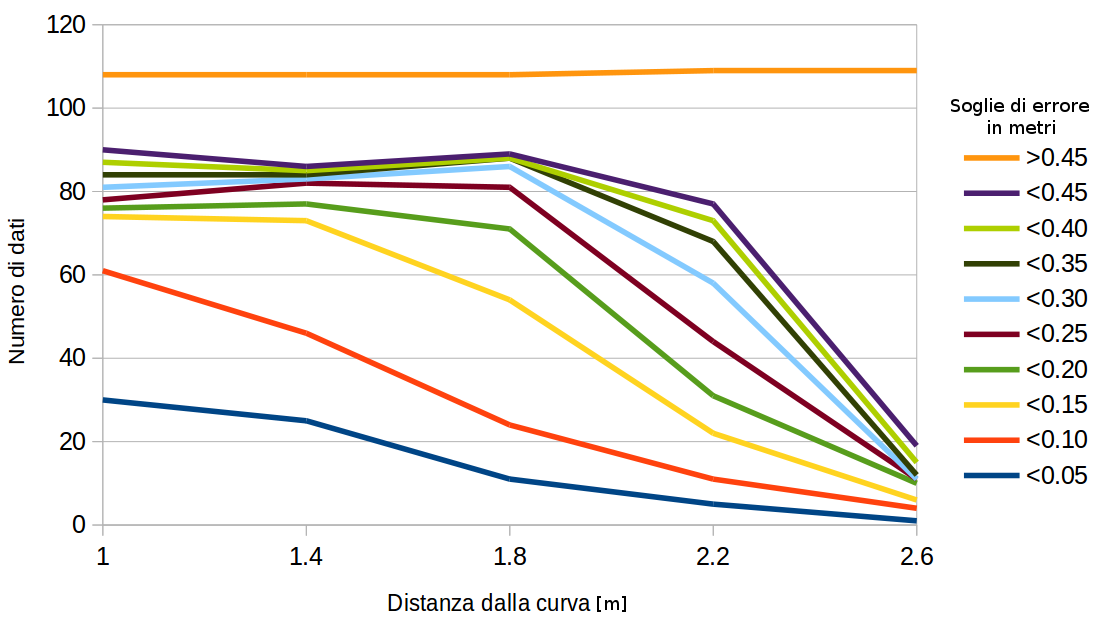
\includegraphics[width=0.7\textwidth]{img/graphradius}
        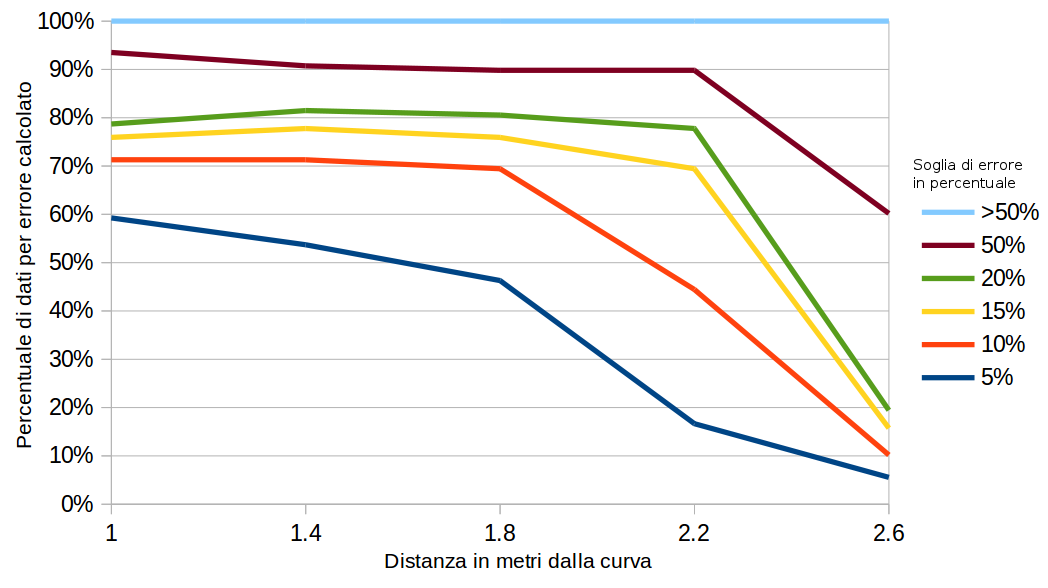
\includegraphics[width=0.7\textwidth]{img/graphdistance}
        \caption[Grafico sulla percentuale di errore in relazione alla distanza dalla curva]{Anche in questo caso è stata calcolata la percentuale d'errore sul raggio e ordinati in base allla percentuale di errore.}
    \end{figure}

    \begin{table}[h]
        \centering
        \begin{tabular}{ccccccc}
            D. curva[m]\textbackslash errore[\%]    & $\le 5\%$   & $\le 10\%$  & $\le 15\%$  & $\le 20\%$  & $\le 50\%$  & $\ge 50\%$ \\
            1.0     & 64    & 13    &  5    & 3     & 16    &  7 \\
            1.4     & 58    & 19    &  7    & 4     & 10    & 10 \\
            1.8	    & 50    & 25    &  7    & 5     & 10    & 11 \\
            2.2     & 18    & 30    & 27    & 9     & 13    & 11 \\
            2.6     &  6    &  5    &  6    & 4     & 44    & 43 \\
            \\
            Err. medio su $\alpha$: & 45\% \\
        \end{tabular}
        \caption{Numero di dati per percentuale di errore sul calcolo, raggruppati in base alla distanza dalla curva.}
    \end{table}

    \'E già stato discusso come sia complesso ottenere la curva completa, infatti l'algoritmo di pathshape risulta veramente affidabile per distanze inferiori ai \textasciitilde 220cm, con distanze massime \textasciitilde 3m. Per questo motivo identificare nell'immagine la curva nella sua interezza risulta essere un evento piuttosto raro. Questo rende il calcolo dell'angolo di curvatura completamente inutile nella maggioranza dei casi, eccettuando i casi limite in cui abbiamo un raggio di curvatura relativamente piccolo ($<1.5$m) e un angolo di curvatura inferiore ai 30°. A questo punto compare però un problema di affidabilità sul calcolo dei valori di raggio e centro dell'arco di curvatura. Avendo infatti dei parametri di questo tipo il numero di punti posizionati sulla curva sarà piuttosto piccolo, ciò provoca fluttuazioni maggiori portando ad errori maggiori nel calcolo.

    I risultati ottenuti sul raggio di curvatura e sul punto di inizio della curva risultano invece più soddisfacenti (Tab. 4.1), infatti riusciamo a raggiungere nel 60\% dei casi una percentuale di errore inferiore al 5\% per dati ottenuti da curve a una istanza di 1 metro. Invece, se cominciamo a considerare valori ottenuti da curve posizionate a una distanza maggiore notiamo che l'errore comincia ad aumentare. Osservando infatti i dati ottenuti da curve tra gli 1.4 e i 2 metri vediamo che meno del 50\% dei dati ha un errore inferiore al 5\%, nonostante ciò si osserva che una percentuale di dati maggiore al 20\% presenta un errore di calcolo tra i 5 e il 10\%. In un ultimo caso osservando i valori calcolati su curve a distanze maggioridi 2 metri notiamo un peggioramento sensibile, con un numero di dati intorno al 40\% che manifesta errori tra il 20\% e il 50\% e un ulteriore 40\% dei dati che risulta errato di più di 50\% del valore.

    Concludendo risultano comunque dati peggiori di quanto sperato. Si nota particolarmente una diminuzione nella precisione del calcolo all'aumentare della distanza dalla curva. Questo è dovuto a un limite attribuibile all'algoritmo di pathshape. Infatti, è stato osservato che a distanze superiori ai 2.5 metri l'algoritmo raramente identifica dei punti all'interno della linea. In aggiunta a ciò i pochi punti ottenuti oltre i 2 metri risultano afflitti da errori, soprattutto se questi vengono identificati all'interno di una curva. La presenza di pochi punti afflitti da errori causa forti problemi nella fase di calcolo dei parametri della curva, portando a delle alterazioni significative nel risultato calcolato.

    \begin{figure}[!ht]
        \centering
        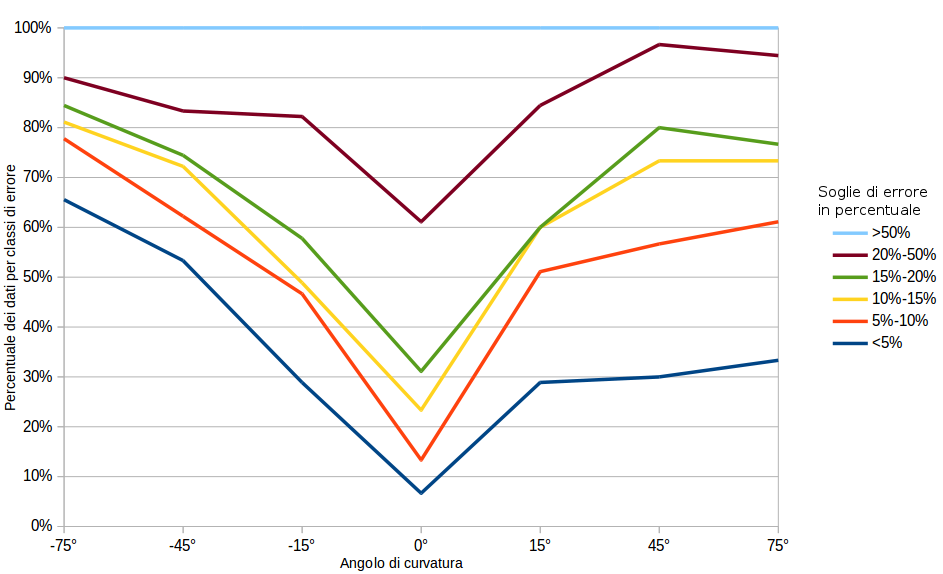
\includegraphics[width=0.75\textwidth]{img/graphangle}
        \caption[Grafico sulla percentuale di errore in relazione all'angolo di curvatura]{La percentuale di errore è stata calcolata comparando il raggio calcolato dall'algoritmo con il raggio noto. \'E quindi stato effettuato un conteggio sul numero di dati in base all'errore.}
    \end{figure}

\section{Test sulla funzione di matching}

    Per verificare le prestazioni ottenute dalla funzione di matching sono stati costruiti una serie di percorsi utilizzando MATLAB, contenenti diverse tipologie di curve. Per ogni curva sono state create circa 3 immagini, ognuna a distanza diversa dalla curva presa in analisi quindi i parametri di ogni curva sono stati inseriti all'interno dell'algoritmo di matching.

    Sono stati testati 5 percorsi differenti, ognuno contenente almeno 5 curve. Le curve avevano diversi raggi e angoli di curvatura per differenziare i vari casi tra di loro e avere un set di testing il più vario possibile.
    \'E importante notare che i parametri delle curve sono stati generati in modo tale da avere un minore numero di alterazioni dovute al comportamento dell'algoritmo di pathshape. Questo ci ha permesso di giudicare l'efficenza della funzione di matching indipendentemente dalle prestazioni dell'algoritmo di pathshape.

    \begin{table}[hb]
        \centering
        \begin{tabular}{ccccc}
            Percorso & Immagini \# & Risultati positivi \# & Successo \% \\
            Percorso 1 & 16 & 14 & 87\% \\
            Percorso 2 & 16 & 14 & 87\% \\
            Percorso 3 & 16 & 12 & 81\% \\
            Percorso 4 & 18 & 17 & 94\% \\
            Percorso 5 & 21 & 19 & 90\% \\
            Totale & 87 &    76 &    87\% \\
        \end{tabular}
        \caption{Risultati ottenuti nei test della funzione di matching, per risultati positivi si intendono in casi in cui l'algoritmo identifica la curva correttamente.}
    \end{table}

    Osservando la Tabella 4.3 si osserva che i risultati ottenuti dalla funzione di matching sono buoni. La curva osservata nell'immagine viene infatti riconosciuta nell'87\% dei casi studiati. Inoltre, è stato riscontrato che nei casi di insuccesso l'errore era causato solitamente da due fattori:
    \begin{itemize}
        \item \textbf{Eccessiva distanza del robot dalla curva:} in alcuni casi ciò comportava un mancato riconoscimento dei punti in curva, in quanto essa risultava essere troppo distante, mentre in altri casi si riscontrava un errore nel calcolo dei parametri della curva dovuto a un numero basso di punti identificati all'interno di essa.
        \item \textbf{Errori dovuti all'algoritmo di pathshape:} in condizioni particolari (solitamente nel caso di curve con un raggio molto basso) l'algoritmo di pathshape manifestava delle forti deviazioni dal percorso, posizionando dei punti in posizioni anche molto lontane dal marker. Questo provoca spesso dei grossi errori nel calcolo, dovuti a questi punti altamente fuorvianti che non riescono a essere corretti nella fase preliminare.
    \end{itemize}
    In altri casi invece si osserva un errore in percorsi in cui vengono inserite curve con parametri molto simili tra loro. Questo avviene perché nel calcolo della distanza la curva identificata risulta vicina a entrambe portando ad avere un riconoscimento errato. Nonostante ciò la curva corretta viene sempre restituita nel set delle curve vicine dalla funzione di matching.

    Concludendo si osservano dei risultati positivi nell'87\% dei test (numero che potrebbe essere portato a \textasciitilde 95\% rimuovendo i dati fuorviati dal pathshape) numero piuttosto soddisfacente.

\section{Confronto tra i tempi di esecuzione dell'algoritmo di pathshape e l'algoritmo di identificazione della curva}

    Raccogliendo i dati sul tempo computazionale necessario è stato possibile ottenere informazioni rilevanti pur eseguendo i test su un hardware molto più potente di quello effettivamente a disposizione, infatti è possibile utilizzari i dati sul tempo di esecuzione dell'algoritmo di pathshape come confronto per i dati sul tempo di esecuzione dell'algoritmo da me proposto.


        \begin{table}[ht]
            \centering
            \begin{tabular}{cccc}
                T.totale[ms] & T.pathshape[ms] & T. id. curva[ms] & Rapporto[\%]\\
                \\
                43.07 & 42.90 & 0.17 & 0.95\% \\
                \\
            \end{tabular}
            \caption{Sommario del tempo necessario per l'esecuzione della parte di algoritmo di identificazione della curva, descritta nel capitolo 3, in rapporto al tempo di esecuzione dell'algoritmo di pathshape.}
        \end{table}

        Possiamo osservare in questo modo che la parte di codice da me proposta ha un tempo di esecuzione che oscilla tra l'1\textperthousand e il 6\textperthousand dell'algoritmo di pathshape, quindi il suo tempo di esecuzione risulta trascurabile.
